% =====================================================================
\chapter{Base de datos}\label{cap:datos}

\section{Requerimientos}
Del levantamiento del informe 1 (ETN-1000) y de lo que la app ya produce, la base debe guardar:
\begin{itemize}
\item la \textbf{telemetría} de las variables (PV, MV) con marca de tiempo: posiciones de los ejes, frecuencias;
\item los \textbf{cambios de estado} de las señales digitales (finales de carrera, relés, garra);
\item los \textbf{ciclos de operación}: cuándo y en qué modo se usó la planta y con qué programa;
\item las \textbf{órdenes} (acciones de control): quién, cuándo, qué, con qué destinos, aceptada o rechazada y por qué;
\item las \textbf{alarmas}: watchdog, paro, falla de homing, fuera de rango\dots;
\item los \textbf{usuarios, roles e ingresos} (registro de sesiones).
\end{itemize}

\section{Del modelo preliminar al modelo normalizado}
\begin{figure}[H]
\centering
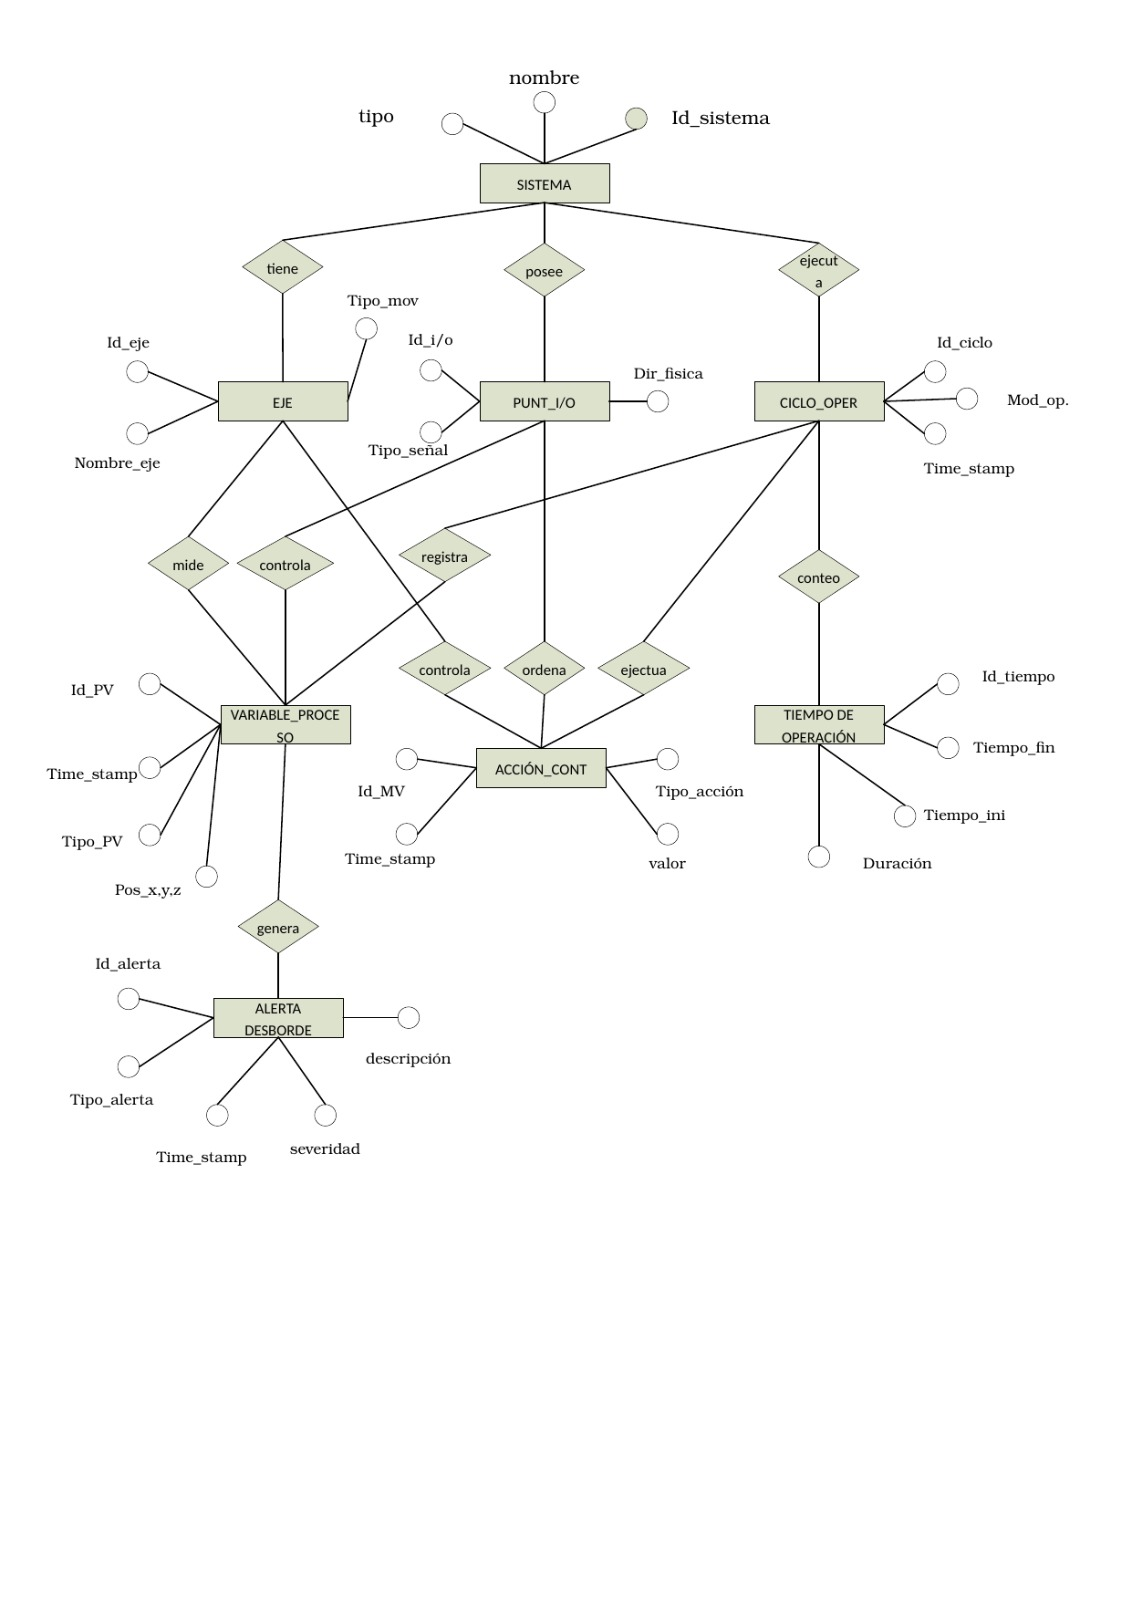
\includegraphics[width=0.62\linewidth, trim=0 360 0 0, clip]{modelo_er_preliminar.png}
\caption{Modelo E-R preliminar del equipo (\texttt{base-de-datos/modelo/}).}
\end{figure}

Cambios para llevarlo a 3FN y a la planta real:
\begin{center}\small
\begin{tabularx}{\linewidth}{>{\raggedright}p{4.4cm} >{\raggedright\arraybackslash}X}
\toprule
\textbf{Preliminar} & \textbf{Normalizado}\\
\midrule
VARIABLE\_PROCESO con \emph{Pos\_x.y.z} & 1FN: un valor por fila; la variable (tag, unidad, rango) está en \codigo{variable} y cada medición en \codigo{muestra}\\
ACCION\_CONT con \emph{valor} & la orden en \codigo{orden}; sus destinos, uno por eje, en \codigo{orden\_parametro} (1FN)\\
TIEMPO DE OPERACIÓN con \emph{Duración} & 3FN: la duración depende de inicio y fin; no se guarda, se calcula en la vista \codigo{v\_ciclo}\\
ALERTA DESBORDE & catálogo \codigo{alarma} (código, severidad) + \codigo{evento\_alarma} (cuándo se activó)\\
PUNT\_I/O & \codigo{punto\_io} con dirección del PLC, tag ISA y eje\\
(no existía) & \codigo{usuario}, \codigo{rol}, \codigo{sesion}: control de acceso y registro de ingresos (guías 3 y Fase 3)\\
(no existía) & \codigo{programa\_plc}: qué programa estaba cargado en cada ciclo\\
\bottomrule
\end{tabularx}
\end{center}

\section{Modelo lógico}\label{sec:tablas}
\begin{figure}[H]
\centering
\begin{tikzpicture}[x=1cm,y=1cm, rel/.style={thick, black!60}, card/.style={font=\tiny\bfseries, fill=white, inner sep=1pt}]
\node[tabla] (sis) at (0,0) {\textbf{sistema}\nodepart{two}PK id\\nombre, tipo, plc};
\node[tabla] (eje) at (4.2,0) {\textbf{eje}\nodepart{two}PK id\\FK sistema\_id\\codigo, nombre, tipo\_mov\\unidad, pulsos\_unidad, lazo\_isa};
\node[tabla] (pio) at (8.4,0) {\textbf{punto\_io}\nodepart{two}PK id\\FK sistema\_id, FK eje\_id\\direccion, tag\_isa (UQ)\\tipo\_senal, descripcion};
\node[tabla] (var) at (4.2,-3.1) {\textbf{variable}\nodepart{two}PK id\\FK eje\_id\\tag\_isa (UQ), clase PV/MV/DV\\nombre, unidad, rango};
\node[tabla] (prog) at (0,-3.1) {\textbf{programa\_plc}\nodepart{two}PK id\\nombre, perfil\_app\\firma, descripcion};
\node[tabla] (ciclo) at (0,-6.2) {\textbf{ciclo\_operacion}\nodepart{two}PK id\\FK sistema\_id\\FK programa\_id\\modo, inicio, fin};
\node[tabla] (mue) at (4.2,-6.2) {\textbf{muestra}\nodepart{two}PK id\\FK ciclo\_id, FK variable\_id\\instante, valor};
\node[tabla] (est) at (8.4,-3.1) {\textbf{estado\_io}\nodepart{two}PK id\\FK ciclo\_id, FK punto\_id\\instante, valor};
\node[tabla] (ord) at (0,-9.3) {\textbf{orden}\nodepart{two}PK id\\FK ciclo\_id, FK usuario\_id\\instante, tipo\\aceptada, motivo};
\node[tabla] (op) at (4.2,-9.3) {\textbf{orden\_parametro}\nodepart{two}PK (orden\_id, eje\_id)\\valor};
\node[tabla] (ala) at (8.4,-9.3) {\textbf{alarma}\nodepart{two}PK id\\codigo (UQ), severidad\\descripcion};
\node[tabla] (eva) at (8.4,-6.2) {\textbf{evento\_alarma}\nodepart{two}PK id\\FK alarma\_id, FK ciclo\_id\\instante, activa, detalle};
\node[tabla] (rol) at (0,-12.2) {\textbf{rol}\nodepart{two}PK id\\nombre (UQ)};
\node[tabla] (usu) at (4.2,-12.2) {\textbf{usuario}\nodepart{two}PK id\\FK rol\_id\\nombre (UQ), clave\_hash};
\node[tabla] (ses) at (8.4,-12.2) {\textbf{sesion}\nodepart{two}PK id\\FK usuario\_id\\ip, instante, exito, fin};
\draw[rel] (sis) -- node[card, pos=0.2]{1} node[card, pos=0.8]{N} (eje);
\draw[rel] (eje) -- node[card, pos=0.2]{1} node[card, pos=0.8]{N} (pio);
\draw[rel] (eje) -- node[card, pos=0.2]{1} node[card, pos=0.8]{N} (var);
\draw[rel] (sis.south west) ++(0.2,0) |- ([yshift=4mm]ciclo.west) ;
\draw[rel] (prog) -- node[card, pos=0.2]{1} node[card, pos=0.8]{N} (ciclo);
\draw[rel] (ciclo) -- node[card, pos=0.2]{1} node[card, pos=0.8]{N} (mue);
\draw[rel] (var) -- node[card, pos=0.2]{1} node[card, pos=0.8]{N} (mue);
\draw[rel] (pio) -- node[card, pos=0.2]{1} node[card, pos=0.8]{N} (est);
\draw[rel] (ciclo.east) ++(0,0.3) -- node[card, pos=0.1]{1} node[card, pos=0.9]{N} (est.west);
\draw[rel] (ciclo) -- node[card, pos=0.2]{1} node[card, pos=0.8]{N} (ord);
\draw[rel] (ord) -- node[card, pos=0.2]{1} node[card, pos=0.8]{N} (op);
\draw[rel] (eje.south east) ++(-0.3,0) -- ++(0,-0.2) -- ([xshift=12mm]op.north);
\draw[rel] (ala) -- node[card, pos=0.2]{1} node[card, pos=0.8]{N} (eva);
\draw[rel] (ciclo.east) ++(0,-0.3) -- (eva.west);
\draw[rel] (rol) -- node[card, pos=0.2]{1} node[card, pos=0.8]{N} (usu);
\draw[rel] (usu) -- node[card, pos=0.2]{1} node[card, pos=0.8]{N} (ses);
\draw[rel] (usu.north west) ++(0.3,0) -- ([xshift=-10mm]ord.south east);
\end{tikzpicture}
\caption{Modelo lógico normalizado (PostgreSQL). PK: clave primaria; FK: clave foránea; UQ: único; 1--N: cardinalidad.}
\end{figure}

\section{Por qué está en tercera forma normal}
\begin{itemize}
\item \textbf{1FN} (valores atómicos, sin grupos repetidos): la posición $(X, Y, Z)$ no va en una celda; cada variable es una fila de \codigo{variable} y cada medición una fila de \codigo{muestra}. Los destinos de una orden van en \codigo{orden\_parametro}, una fila por eje.
\item \textbf{2FN} (sin dependencias parciales): todas las tablas tienen clave simple salvo \codigo{orden\_parametro}, cuyo único atributo \codigo{valor} depende de la clave completa (orden y eje).
\item \textbf{3FN} (sin dependencias transitivas): la unidad y el rango dependen de la variable, no de la muestra; el rol depende del usuario, no de la sesión; la duración de un ciclo depende de inicio y fin y por eso se calcula.
\end{itemize}

\section{El script SQL}
El script \codigo{base-de-datos/scripts/brazo\_4gdl.sql} crea las 15 tablas con sus restricciones, un trigger, dos vistas y carga los datos fijos de la planta: sistema, 4 ejes, 22 señales del PLC con sus tags ISA, 5 variables, 3 programas, 8 alarmas y 2 roles. El listado completo está en el apéndice \ref{ap:sql}.

\begin{lstlisting}[style=sql, caption={Trigger que rechaza muestras fuera de rango (lo pide la guía 1 para la Fase 2).}]
CREATE FUNCTION validar_muestra() RETURNS trigger AS $$
DECLARE
    r variable%ROWTYPE;
BEGIN
    SELECT * INTO r FROM variable WHERE id = NEW.variable_id;
    IF NEW.valor < r.rango_min OR NEW.valor > r.rango_max THEN
        RAISE EXCEPTION 'muestra fuera de rango para % (%): % no está en [%, %]',
            r.tag_isa, r.unidad, NEW.valor, r.rango_min, r.rango_max;
    END IF;
    RETURN NEW;
END;
$$ LANGUAGE plpgsql;
CREATE TRIGGER muestra_en_rango BEFORE INSERT OR UPDATE ON muestra
    FOR EACH ROW EXECUTE FUNCTION validar_muestra();
\end{lstlisting}

\section{De la app a las tablas}
\begin{center}\small
\begin{tabularx}{\linewidth}{>{\raggedright}p{5.4cm} >{\raggedright\arraybackslash}X}
\toprule
\textbf{Dato que ya produce la app} & \textbf{Tabla}\\
\midrule
cambio de modo en el menú & \codigo{ciclo\_operacion} (inicio/fin, modo, programa reconocido)\\
\codigo{/api/estado}: \codigo{theta\_deg}, \codigo{sX\_mm}, \codigo{sY\_mm} & \codigo{muestra} con las variables ZI-101, ZI-102, ZI-103\\
\codigo{/api/estado}: entradas y salidas & \codigo{estado\_io} (solo los cambios)\\
línea \codigo{orden mover \{...\} (usuario)} del registro & \codigo{orden} + \codigo{orden\_parametro}\\
línea \codigo{RECHAZADO ...} & \codigo{orden} con \codigo{aceptada = false} y su motivo\\
error del PLC (VB1123), pérdida de comunicación & \codigo{evento\_alarma}\\
\codigo{usuarios.json} & \codigo{usuario} y \codigo{rol} (mismo hash PBKDF2)\\
líneas \codigo{ingreso de ...} / \codigo{ingreso fallido} & \codigo{sesion}\\
\bottomrule
\end{tabularx}
\end{center}

\begin{lstlisting}[style=sql, caption={Consultas de ejemplo.}]
-- Posición del carro X en el último ciclo, cada segundo
SELECT date_trunc('second', m.instante) AS t, avg(m.valor) AS x_mm
FROM muestra m JOIN variable v ON v.id = m.variable_id
WHERE v.tag_isa = 'ZI-102' AND m.ciclo_id = (SELECT max(id) FROM ciclo_operacion)
GROUP BY 1 ORDER BY 1;

-- Órdenes rechazadas por usuario y motivo
SELECT u.nombre, o.motivo, count(*) FROM orden o LEFT JOIN usuario u ON u.id = o.usuario_id
WHERE NOT o.aceptada GROUP BY 1, 2 ORDER BY 3 DESC;
\end{lstlisting}

\pendiente{El script no se ejecutó todavía: la PC donde se escribió no tiene PostgreSQL. Falta: (1) crear la base y correr el script en la PC del laboratorio; (2) agregar a la app un módulo que inserte las muestras (por ejemplo, una por segundo y por eje), los cambios de E/S, las órdenes y los ingresos, con la biblioteca \codigo{psycopg}; (3) un tablero que consulte el historial.}
